\documentclass[twoside]{book}

% Packages required by doxygen
\usepackage{fixltx2e}
\usepackage{calc}
\usepackage{doxygen}
\usepackage[export]{adjustbox} % also loads graphicx
\usepackage{graphicx}
\usepackage[utf8]{inputenc}
\usepackage{makeidx}
\usepackage{multicol}
\usepackage{multirow}
\PassOptionsToPackage{warn}{textcomp}
\usepackage{textcomp}
\usepackage[nointegrals]{wasysym}
\usepackage[table]{xcolor}

% Font selection
\usepackage[T1]{fontenc}
\usepackage[scaled=.90]{helvet}
\usepackage{courier}
\usepackage{amssymb}
\usepackage{sectsty}
\renewcommand{\familydefault}{\sfdefault}
\allsectionsfont{%
  \fontseries{bc}\selectfont%
  \color{darkgray}%
}
\renewcommand{\DoxyLabelFont}{%
  \fontseries{bc}\selectfont%
  \color{darkgray}%
}
\newcommand{\+}{\discretionary{\mbox{\scriptsize$\hookleftarrow$}}{}{}}

% Page & text layout
\usepackage{geometry}
\geometry{%
  a4paper,%
  top=2.5cm,%
  bottom=2.5cm,%
  left=2.5cm,%
  right=2.5cm%
}
\tolerance=750
\hfuzz=15pt
\hbadness=750
\setlength{\emergencystretch}{15pt}
\setlength{\parindent}{0cm}
\setlength{\parskip}{3ex plus 2ex minus 2ex}
\makeatletter
\renewcommand{\paragraph}{%
  \@startsection{paragraph}{4}{0ex}{-1.0ex}{1.0ex}{%
    \normalfont\normalsize\bfseries\SS@parafont%
  }%
}
\renewcommand{\subparagraph}{%
  \@startsection{subparagraph}{5}{0ex}{-1.0ex}{1.0ex}{%
    \normalfont\normalsize\bfseries\SS@subparafont%
  }%
}
\makeatother

% Headers & footers
\usepackage{fancyhdr}
\pagestyle{fancyplain}
\fancyhead[LE]{\fancyplain{}{\bfseries\thepage}}
\fancyhead[CE]{\fancyplain{}{}}
\fancyhead[RE]{\fancyplain{}{\bfseries\leftmark}}
\fancyhead[LO]{\fancyplain{}{\bfseries\rightmark}}
\fancyhead[CO]{\fancyplain{}{}}
\fancyhead[RO]{\fancyplain{}{\bfseries\thepage}}
\fancyfoot[LE]{\fancyplain{}{}}
\fancyfoot[CE]{\fancyplain{}{}}
\fancyfoot[RE]{\fancyplain{}{\bfseries\scriptsize Generated by Doxygen }}
\fancyfoot[LO]{\fancyplain{}{\bfseries\scriptsize Generated by Doxygen }}
\fancyfoot[CO]{\fancyplain{}{}}
\fancyfoot[RO]{\fancyplain{}{}}
\renewcommand{\footrulewidth}{0.4pt}
\renewcommand{\chaptermark}[1]{%
  \markboth{#1}{}%
}
\renewcommand{\sectionmark}[1]{%
  \markright{\thesection\ #1}%
}

% Indices & bibliography
\usepackage{natbib}
\usepackage[titles]{tocloft}
\setcounter{tocdepth}{3}
\setcounter{secnumdepth}{5}
\makeindex

% Hyperlinks (required, but should be loaded last)
\usepackage{ifpdf}
\ifpdf
  \usepackage[pdftex,pagebackref=true]{hyperref}
\else
  \usepackage[ps2pdf,pagebackref=true]{hyperref}
\fi
\hypersetup{%
  colorlinks=true,%
  linkcolor=blue,%
  citecolor=blue,%
  unicode%
}

% Custom commands
\newcommand{\clearemptydoublepage}{%
  \newpage{\pagestyle{empty}\cleardoublepage}%
}

\usepackage{caption}
\captionsetup{labelsep=space,justification=centering,font={bf},singlelinecheck=off,skip=4pt,position=top}

%===== C O N T E N T S =====

\begin{document}

% Titlepage & ToC
\hypersetup{pageanchor=false,
             bookmarksnumbered=true,
             pdfencoding=unicode
            }
\pagenumbering{alph}
\begin{titlepage}
\vspace*{7cm}
\begin{center}%
{\Large My Noob Project }\\
\vspace*{1cm}
{\large Generated by Doxygen 1.8.15}\\
\end{center}
\end{titlepage}
\clearemptydoublepage
\pagenumbering{roman}
\tableofcontents
\clearemptydoublepage
\pagenumbering{arabic}
\hypersetup{pageanchor=true}

%--- Begin generated contents ---
\chapter{Hierarchical Index}
\section{Class Hierarchy}
This inheritance list is sorted roughly, but not completely, alphabetically\+:\begin{DoxyCompactList}
\item \contentsline{section}{com.\+example.\+victorardianto.\+myapplication.\+model.\+Cinema\+Seat}{\pageref{classcom_1_1example_1_1victorardianto_1_1myapplication_1_1model_1_1_cinema_seat}}{}
\item \contentsline{section}{com.\+example.\+victorardianto.\+myapplication.\+model.\+Cinema\+Seat\+Identity}{\pageref{classcom_1_1example_1_1victorardianto_1_1myapplication_1_1model_1_1_cinema_seat_identity}}{}
\item App\+Compat\+Activity\begin{DoxyCompactList}
\item \contentsline{section}{com.\+example.\+victorardianto.\+myapplication.\+Main\+Activity}{\pageref{classcom_1_1example_1_1victorardianto_1_1myapplication_1_1_main_activity}}{}
\end{DoxyCompactList}
\item Frame\+Layout\begin{DoxyCompactList}
\item \contentsline{section}{com.\+example.\+victorardianto.\+myapplication.\+widget.\+Two\+D\+Scroll\+Frame\+Layout}{\pageref{classcom_1_1example_1_1victorardianto_1_1myapplication_1_1widget_1_1_two_d_scroll_frame_layout}}{}
\item \contentsline{section}{com.\+example.\+victorardianto.\+myapplication.\+widget.\+Two\+D\+Scroll\+View}{\pageref{classcom_1_1example_1_1victorardianto_1_1myapplication_1_1widget_1_1_two_d_scroll_view}}{}
\end{DoxyCompactList}
\end{DoxyCompactList}

\chapter{Class Index}
\section{Class List}
Here are the classes, structs, unions and interfaces with brief descriptions\+:\begin{DoxyCompactList}
\item\contentsline{section}{\mbox{\hyperlink{classcom_1_1example_1_1victorardianto_1_1myapplication_1_1model_1_1_cinema_seat}{com.\+example.\+victorardianto.\+myapplication.\+model.\+Cinema\+Seat}} }{\pageref{classcom_1_1example_1_1victorardianto_1_1myapplication_1_1model_1_1_cinema_seat}}{}
\item\contentsline{section}{\mbox{\hyperlink{classcom_1_1example_1_1victorardianto_1_1myapplication_1_1model_1_1_cinema_seat_identity}{com.\+example.\+victorardianto.\+myapplication.\+model.\+Cinema\+Seat\+Identity}} }{\pageref{classcom_1_1example_1_1victorardianto_1_1myapplication_1_1model_1_1_cinema_seat_identity}}{}
\item\contentsline{section}{\mbox{\hyperlink{classcom_1_1example_1_1victorardianto_1_1myapplication_1_1_main_activity}{com.\+example.\+victorardianto.\+myapplication.\+Main\+Activity}} }{\pageref{classcom_1_1example_1_1victorardianto_1_1myapplication_1_1_main_activity}}{}
\item\contentsline{section}{\mbox{\hyperlink{classcom_1_1example_1_1victorardianto_1_1myapplication_1_1widget_1_1_two_d_scroll_frame_layout}{com.\+example.\+victorardianto.\+myapplication.\+widget.\+Two\+D\+Scroll\+Frame\+Layout}} }{\pageref{classcom_1_1example_1_1victorardianto_1_1myapplication_1_1widget_1_1_two_d_scroll_frame_layout}}{}
\item\contentsline{section}{\mbox{\hyperlink{classcom_1_1example_1_1victorardianto_1_1myapplication_1_1widget_1_1_two_d_scroll_view}{com.\+example.\+victorardianto.\+myapplication.\+widget.\+Two\+D\+Scroll\+View}} }{\pageref{classcom_1_1example_1_1victorardianto_1_1myapplication_1_1widget_1_1_two_d_scroll_view}}{}
\end{DoxyCompactList}

\chapter{Class Documentation}
\hypertarget{classcom_1_1example_1_1victorardianto_1_1myapplication_1_1model_1_1_cinema_seat}{}\section{com.\+example.\+victorardianto.\+myapplication.\+model.\+Cinema\+Seat Class Reference}
\label{classcom_1_1example_1_1victorardianto_1_1myapplication_1_1model_1_1_cinema_seat}\index{com.\+example.\+victorardianto.\+myapplication.\+model.\+Cinema\+Seat@{com.\+example.\+victorardianto.\+myapplication.\+model.\+Cinema\+Seat}}
\subsection*{Public Member Functions}
\begin{DoxyCompactItemize}
\item 
\mbox{\Hypertarget{classcom_1_1example_1_1victorardianto_1_1myapplication_1_1model_1_1_cinema_seat_af5376bd5edc4756f9e04dea62e47f9b1}\label{classcom_1_1example_1_1victorardianto_1_1myapplication_1_1model_1_1_cinema_seat_af5376bd5edc4756f9e04dea62e47f9b1}} 
\mbox{\hyperlink{classcom_1_1example_1_1victorardianto_1_1myapplication_1_1model_1_1_cinema_seat_identity}{Cinema\+Seat\+Identity}} {\bfseries get\+Identity} ()
\item 
\mbox{\Hypertarget{classcom_1_1example_1_1victorardianto_1_1myapplication_1_1model_1_1_cinema_seat_a04c3b1060a359aef2db6a207df4f4098}\label{classcom_1_1example_1_1victorardianto_1_1myapplication_1_1model_1_1_cinema_seat_a04c3b1060a359aef2db6a207df4f4098}} 
void {\bfseries set\+Identity} (\mbox{\hyperlink{classcom_1_1example_1_1victorardianto_1_1myapplication_1_1model_1_1_cinema_seat_identity}{Cinema\+Seat\+Identity}} identity)
\item 
\mbox{\Hypertarget{classcom_1_1example_1_1victorardianto_1_1myapplication_1_1model_1_1_cinema_seat_ac91dd9631d78ecc64e9cab067502fabf}\label{classcom_1_1example_1_1victorardianto_1_1myapplication_1_1model_1_1_cinema_seat_ac91dd9631d78ecc64e9cab067502fabf}} 
int {\bfseries get\+Text\+Color} ()
\item 
\mbox{\Hypertarget{classcom_1_1example_1_1victorardianto_1_1myapplication_1_1model_1_1_cinema_seat_a35b214dab3ebd74ed36c5a556a57f2d5}\label{classcom_1_1example_1_1victorardianto_1_1myapplication_1_1model_1_1_cinema_seat_a35b214dab3ebd74ed36c5a556a57f2d5}} 
int {\bfseries get\+Fill\+Color} ()
\end{DoxyCompactItemize}


\subsection{Detailed Description}
Created by victorardianto on 30/01/18. 

Definition at line 9 of file Cinema\+Seat.\+java.



The documentation for this class was generated from the following file\+:\begin{DoxyCompactItemize}
\item 
com/example/victorardianto/myapplication/model/Cinema\+Seat.\+java\end{DoxyCompactItemize}

\hypertarget{classcom_1_1example_1_1victorardianto_1_1myapplication_1_1model_1_1_cinema_seat_identity}{}\section{com.\+example.\+victorardianto.\+myapplication.\+model.\+Cinema\+Seat\+Identity Class Reference}
\label{classcom_1_1example_1_1victorardianto_1_1myapplication_1_1model_1_1_cinema_seat_identity}\index{com.\+example.\+victorardianto.\+myapplication.\+model.\+Cinema\+Seat\+Identity@{com.\+example.\+victorardianto.\+myapplication.\+model.\+Cinema\+Seat\+Identity}}
\subsection*{Public Member Functions}
\begin{DoxyCompactItemize}
\item 
\mbox{\Hypertarget{classcom_1_1example_1_1victorardianto_1_1myapplication_1_1model_1_1_cinema_seat_identity_ae49dd73693482dd50c11ca8a1a55e343}\label{classcom_1_1example_1_1victorardianto_1_1myapplication_1_1model_1_1_cinema_seat_identity_ae49dd73693482dd50c11ca8a1a55e343}} 
{\bfseries Cinema\+Seat\+Identity} (String number, int position)
\item 
\mbox{\Hypertarget{classcom_1_1example_1_1victorardianto_1_1myapplication_1_1model_1_1_cinema_seat_identity_ad8374b68303e554835471cd728d1b43a}\label{classcom_1_1example_1_1victorardianto_1_1myapplication_1_1model_1_1_cinema_seat_identity_ad8374b68303e554835471cd728d1b43a}} 
String {\bfseries get\+Number} ()
\item 
\mbox{\Hypertarget{classcom_1_1example_1_1victorardianto_1_1myapplication_1_1model_1_1_cinema_seat_identity_ab0171e74db066d10e467dd2dbeda1e7f}\label{classcom_1_1example_1_1victorardianto_1_1myapplication_1_1model_1_1_cinema_seat_identity_ab0171e74db066d10e467dd2dbeda1e7f}} 
int {\bfseries get\+Position} ()
\end{DoxyCompactItemize}


\subsection{Detailed Description}
Created by victorardianto on 30/01/18. 

Definition at line 7 of file Cinema\+Seat\+Identity.\+java.



The documentation for this class was generated from the following file\+:\begin{DoxyCompactItemize}
\item 
com/example/victorardianto/myapplication/model/Cinema\+Seat\+Identity.\+java\end{DoxyCompactItemize}

\hypertarget{classcom_1_1example_1_1victorardianto_1_1myapplication_1_1_main_activity}{}\section{com.\+example.\+victorardianto.\+myapplication.\+Main\+Activity Class Reference}
\label{classcom_1_1example_1_1victorardianto_1_1myapplication_1_1_main_activity}\index{com.\+example.\+victorardianto.\+myapplication.\+Main\+Activity@{com.\+example.\+victorardianto.\+myapplication.\+Main\+Activity}}
Inheritance diagram for com.\+example.\+victorardianto.\+myapplication.\+Main\+Activity\+:\begin{figure}[H]
\begin{center}
\leavevmode
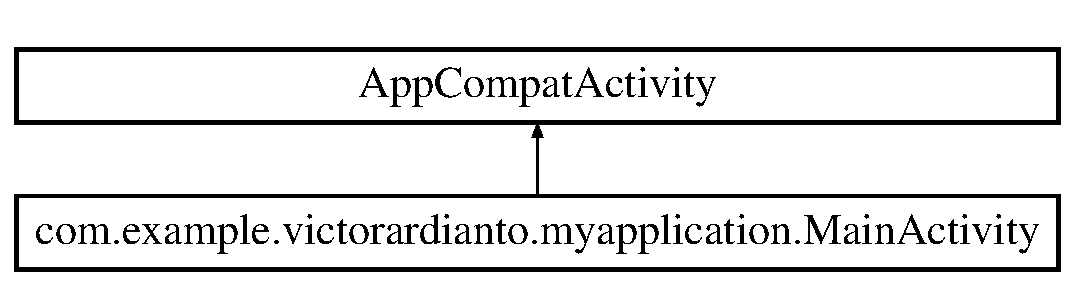
\includegraphics[height=2.000000cm]{classcom_1_1example_1_1victorardianto_1_1myapplication_1_1_main_activity}
\end{center}
\end{figure}
\subsection*{Protected Member Functions}
\begin{DoxyCompactItemize}
\item 
\mbox{\Hypertarget{classcom_1_1example_1_1victorardianto_1_1myapplication_1_1_main_activity_a23f04dd111a1fdb9b5675a9e0eccba70}\label{classcom_1_1example_1_1victorardianto_1_1myapplication_1_1_main_activity_a23f04dd111a1fdb9b5675a9e0eccba70}} 
void {\bfseries on\+Create} (Bundle saved\+Instance\+State)
\end{DoxyCompactItemize}


\subsection{Detailed Description}
The type Main activity. 

Definition at line 26 of file Main\+Activity.\+java.



The documentation for this class was generated from the following file\+:\begin{DoxyCompactItemize}
\item 
com/example/victorardianto/myapplication/Main\+Activity.\+java\end{DoxyCompactItemize}

\hypertarget{classcom_1_1example_1_1victorardianto_1_1myapplication_1_1widget_1_1_two_d_scroll_frame_layout}{}\section{com.\+example.\+victorardianto.\+myapplication.\+widget.\+Two\+D\+Scroll\+Frame\+Layout Class Reference}
\label{classcom_1_1example_1_1victorardianto_1_1myapplication_1_1widget_1_1_two_d_scroll_frame_layout}\index{com.\+example.\+victorardianto.\+myapplication.\+widget.\+Two\+D\+Scroll\+Frame\+Layout@{com.\+example.\+victorardianto.\+myapplication.\+widget.\+Two\+D\+Scroll\+Frame\+Layout}}
Inheritance diagram for com.\+example.\+victorardianto.\+myapplication.\+widget.\+Two\+D\+Scroll\+Frame\+Layout\+:\begin{figure}[H]
\begin{center}
\leavevmode
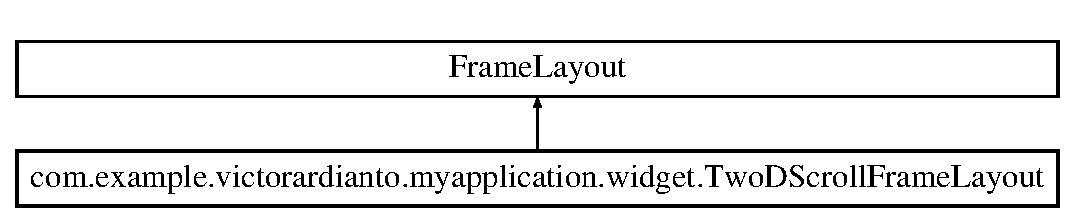
\includegraphics[height=2.000000cm]{classcom_1_1example_1_1victorardianto_1_1myapplication_1_1widget_1_1_two_d_scroll_frame_layout}
\end{center}
\end{figure}
\subsection*{Public Member Functions}
\begin{DoxyCompactItemize}
\item 
\mbox{\hyperlink{classcom_1_1example_1_1victorardianto_1_1myapplication_1_1widget_1_1_two_d_scroll_frame_layout_a7203f0c9e2344b39fbbd36f169ebeca7}{Two\+D\+Scroll\+Frame\+Layout}} (@Non\+Null Context context)
\item 
\mbox{\hyperlink{classcom_1_1example_1_1victorardianto_1_1myapplication_1_1widget_1_1_two_d_scroll_frame_layout_ae59c58441dd9b1653cd43e4159b700c7}{Two\+D\+Scroll\+Frame\+Layout}} (@Non\+Null Context context, @Nullable Attribute\+Set attrs)
\item 
\mbox{\hyperlink{classcom_1_1example_1_1victorardianto_1_1myapplication_1_1widget_1_1_two_d_scroll_frame_layout_a52b4b0fff06dc926b6cfde22d9e4e1de}{Two\+D\+Scroll\+Frame\+Layout}} (@Non\+Null Context context, @Nullable Attribute\+Set attrs, int def\+Style\+Attr)
\item 
\mbox{\Hypertarget{classcom_1_1example_1_1victorardianto_1_1myapplication_1_1widget_1_1_two_d_scroll_frame_layout_ac8921e7ddf806fbf3549c1373fe6f519}\label{classcom_1_1example_1_1victorardianto_1_1myapplication_1_1widget_1_1_two_d_scroll_frame_layout_ac8921e7ddf806fbf3549c1373fe6f519}} 
boolean {\bfseries on\+Intercept\+Touch\+Event} (Motion\+Event ev)
\item 
\mbox{\Hypertarget{classcom_1_1example_1_1victorardianto_1_1myapplication_1_1widget_1_1_two_d_scroll_frame_layout_a6fdc5fe1d7ee0bc2394c328f8a3fd5c8}\label{classcom_1_1example_1_1victorardianto_1_1myapplication_1_1widget_1_1_two_d_scroll_frame_layout_a6fdc5fe1d7ee0bc2394c328f8a3fd5c8}} 
boolean {\bfseries on\+Touch\+Event} (Motion\+Event ev)
\end{DoxyCompactItemize}
\subsection*{Protected Member Functions}
\begin{DoxyCompactItemize}
\item 
void \mbox{\hyperlink{classcom_1_1example_1_1victorardianto_1_1myapplication_1_1widget_1_1_two_d_scroll_frame_layout_a88d422887ecec9da3f0999127b499004}{init\+Two\+D\+Scroll\+View}} ()
\item 
\mbox{\Hypertarget{classcom_1_1example_1_1victorardianto_1_1myapplication_1_1widget_1_1_two_d_scroll_frame_layout_a1b2998b3884b56aebca5fd2c90bb206c}\label{classcom_1_1example_1_1victorardianto_1_1myapplication_1_1widget_1_1_two_d_scroll_frame_layout_a1b2998b3884b56aebca5fd2c90bb206c}} 
void {\bfseries measure\+Child\+With\+Margins} (View child, int parent\+Width\+Measure\+Spec, int width\+Used, int parent\+Height\+Measure\+Spec, int height\+Used)
\end{DoxyCompactItemize}


\subsection{Detailed Description}
Created by victorardianto on 31/01/18. 

Definition at line 16 of file Two\+D\+Scroll\+Frame\+Layout.\+java.



\subsection{Constructor \& Destructor Documentation}
\mbox{\Hypertarget{classcom_1_1example_1_1victorardianto_1_1myapplication_1_1widget_1_1_two_d_scroll_frame_layout_a7203f0c9e2344b39fbbd36f169ebeca7}\label{classcom_1_1example_1_1victorardianto_1_1myapplication_1_1widget_1_1_two_d_scroll_frame_layout_a7203f0c9e2344b39fbbd36f169ebeca7}} 
\index{com\+::example\+::victorardianto\+::myapplication\+::widget\+::\+Two\+D\+Scroll\+Frame\+Layout@{com\+::example\+::victorardianto\+::myapplication\+::widget\+::\+Two\+D\+Scroll\+Frame\+Layout}!Two\+D\+Scroll\+Frame\+Layout@{Two\+D\+Scroll\+Frame\+Layout}}
\index{Two\+D\+Scroll\+Frame\+Layout@{Two\+D\+Scroll\+Frame\+Layout}!com\+::example\+::victorardianto\+::myapplication\+::widget\+::\+Two\+D\+Scroll\+Frame\+Layout@{com\+::example\+::victorardianto\+::myapplication\+::widget\+::\+Two\+D\+Scroll\+Frame\+Layout}}
\subsubsection{\texorpdfstring{Two\+D\+Scroll\+Frame\+Layout()}{TwoDScrollFrameLayout()}\hspace{0.1cm}{\footnotesize\ttfamily [1/3]}}
{\footnotesize\ttfamily com.\+example.\+victorardianto.\+myapplication.\+widget.\+Two\+D\+Scroll\+Frame\+Layout.\+Two\+D\+Scroll\+Frame\+Layout (\begin{DoxyParamCaption}\item[{@Non\+Null Context}]{context }\end{DoxyParamCaption})\hspace{0.3cm}{\ttfamily [inline]}}

Instantiates a new Two d scroll frame layout.


\begin{DoxyParams}{Parameters}
{\em context} & the context \\
\hline
\end{DoxyParams}


Definition at line 30 of file Two\+D\+Scroll\+Frame\+Layout.\+java.

\mbox{\Hypertarget{classcom_1_1example_1_1victorardianto_1_1myapplication_1_1widget_1_1_two_d_scroll_frame_layout_ae59c58441dd9b1653cd43e4159b700c7}\label{classcom_1_1example_1_1victorardianto_1_1myapplication_1_1widget_1_1_two_d_scroll_frame_layout_ae59c58441dd9b1653cd43e4159b700c7}} 
\index{com\+::example\+::victorardianto\+::myapplication\+::widget\+::\+Two\+D\+Scroll\+Frame\+Layout@{com\+::example\+::victorardianto\+::myapplication\+::widget\+::\+Two\+D\+Scroll\+Frame\+Layout}!Two\+D\+Scroll\+Frame\+Layout@{Two\+D\+Scroll\+Frame\+Layout}}
\index{Two\+D\+Scroll\+Frame\+Layout@{Two\+D\+Scroll\+Frame\+Layout}!com\+::example\+::victorardianto\+::myapplication\+::widget\+::\+Two\+D\+Scroll\+Frame\+Layout@{com\+::example\+::victorardianto\+::myapplication\+::widget\+::\+Two\+D\+Scroll\+Frame\+Layout}}
\subsubsection{\texorpdfstring{Two\+D\+Scroll\+Frame\+Layout()}{TwoDScrollFrameLayout()}\hspace{0.1cm}{\footnotesize\ttfamily [2/3]}}
{\footnotesize\ttfamily com.\+example.\+victorardianto.\+myapplication.\+widget.\+Two\+D\+Scroll\+Frame\+Layout.\+Two\+D\+Scroll\+Frame\+Layout (\begin{DoxyParamCaption}\item[{@Non\+Null Context}]{context,  }\item[{@Nullable Attribute\+Set}]{attrs }\end{DoxyParamCaption})\hspace{0.3cm}{\ttfamily [inline]}}

Instantiates a new Two d scroll frame layout.


\begin{DoxyParams}{Parameters}
{\em context} & the context \\
\hline
{\em attrs} & the attrs \\
\hline
\end{DoxyParams}


Definition at line 41 of file Two\+D\+Scroll\+Frame\+Layout.\+java.

\mbox{\Hypertarget{classcom_1_1example_1_1victorardianto_1_1myapplication_1_1widget_1_1_two_d_scroll_frame_layout_a52b4b0fff06dc926b6cfde22d9e4e1de}\label{classcom_1_1example_1_1victorardianto_1_1myapplication_1_1widget_1_1_two_d_scroll_frame_layout_a52b4b0fff06dc926b6cfde22d9e4e1de}} 
\index{com\+::example\+::victorardianto\+::myapplication\+::widget\+::\+Two\+D\+Scroll\+Frame\+Layout@{com\+::example\+::victorardianto\+::myapplication\+::widget\+::\+Two\+D\+Scroll\+Frame\+Layout}!Two\+D\+Scroll\+Frame\+Layout@{Two\+D\+Scroll\+Frame\+Layout}}
\index{Two\+D\+Scroll\+Frame\+Layout@{Two\+D\+Scroll\+Frame\+Layout}!com\+::example\+::victorardianto\+::myapplication\+::widget\+::\+Two\+D\+Scroll\+Frame\+Layout@{com\+::example\+::victorardianto\+::myapplication\+::widget\+::\+Two\+D\+Scroll\+Frame\+Layout}}
\subsubsection{\texorpdfstring{Two\+D\+Scroll\+Frame\+Layout()}{TwoDScrollFrameLayout()}\hspace{0.1cm}{\footnotesize\ttfamily [3/3]}}
{\footnotesize\ttfamily com.\+example.\+victorardianto.\+myapplication.\+widget.\+Two\+D\+Scroll\+Frame\+Layout.\+Two\+D\+Scroll\+Frame\+Layout (\begin{DoxyParamCaption}\item[{@Non\+Null Context}]{context,  }\item[{@Nullable Attribute\+Set}]{attrs,  }\item[{int}]{def\+Style\+Attr }\end{DoxyParamCaption})\hspace{0.3cm}{\ttfamily [inline]}}

Instantiates a new Two d scroll frame layout.


\begin{DoxyParams}{Parameters}
{\em context} & the context \\
\hline
{\em attrs} & the attrs \\
\hline
{\em def\+Style\+Attr} & the def style attr \\
\hline
\end{DoxyParams}


Definition at line 53 of file Two\+D\+Scroll\+Frame\+Layout.\+java.



\subsection{Member Function Documentation}
\mbox{\Hypertarget{classcom_1_1example_1_1victorardianto_1_1myapplication_1_1widget_1_1_two_d_scroll_frame_layout_a88d422887ecec9da3f0999127b499004}\label{classcom_1_1example_1_1victorardianto_1_1myapplication_1_1widget_1_1_two_d_scroll_frame_layout_a88d422887ecec9da3f0999127b499004}} 
\index{com\+::example\+::victorardianto\+::myapplication\+::widget\+::\+Two\+D\+Scroll\+Frame\+Layout@{com\+::example\+::victorardianto\+::myapplication\+::widget\+::\+Two\+D\+Scroll\+Frame\+Layout}!init\+Two\+D\+Scroll\+View@{init\+Two\+D\+Scroll\+View}}
\index{init\+Two\+D\+Scroll\+View@{init\+Two\+D\+Scroll\+View}!com\+::example\+::victorardianto\+::myapplication\+::widget\+::\+Two\+D\+Scroll\+Frame\+Layout@{com\+::example\+::victorardianto\+::myapplication\+::widget\+::\+Two\+D\+Scroll\+Frame\+Layout}}
\subsubsection{\texorpdfstring{init\+Two\+D\+Scroll\+View()}{initTwoDScrollView()}}
{\footnotesize\ttfamily void com.\+example.\+victorardianto.\+myapplication.\+widget.\+Two\+D\+Scroll\+Frame\+Layout.\+init\+Two\+D\+Scroll\+View (\begin{DoxyParamCaption}{ }\end{DoxyParamCaption})\hspace{0.3cm}{\ttfamily [inline]}, {\ttfamily [protected]}}

Init two d scroll view. 

Definition at line 61 of file Two\+D\+Scroll\+Frame\+Layout.\+java.



The documentation for this class was generated from the following file\+:\begin{DoxyCompactItemize}
\item 
com/example/victorardianto/myapplication/widget/Two\+D\+Scroll\+Frame\+Layout.\+java\end{DoxyCompactItemize}

\hypertarget{classcom_1_1example_1_1victorardianto_1_1myapplication_1_1widget_1_1_two_d_scroll_view}{}\section{com.\+example.\+victorardianto.\+myapplication.\+widget.\+Two\+D\+Scroll\+View Class Reference}
\label{classcom_1_1example_1_1victorardianto_1_1myapplication_1_1widget_1_1_two_d_scroll_view}\index{com.\+example.\+victorardianto.\+myapplication.\+widget.\+Two\+D\+Scroll\+View@{com.\+example.\+victorardianto.\+myapplication.\+widget.\+Two\+D\+Scroll\+View}}
Inheritance diagram for com.\+example.\+victorardianto.\+myapplication.\+widget.\+Two\+D\+Scroll\+View\+:\begin{figure}[H]
\begin{center}
\leavevmode
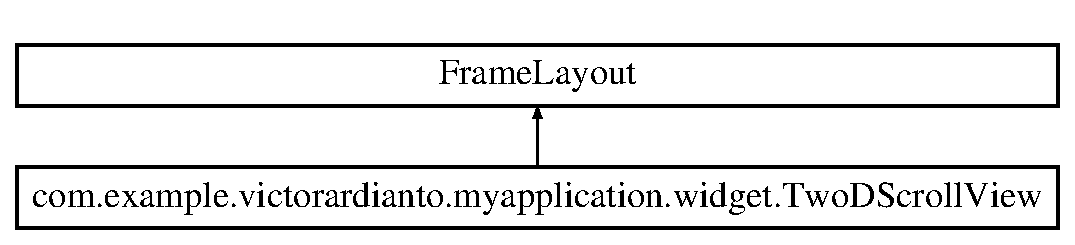
\includegraphics[height=2.000000cm]{classcom_1_1example_1_1victorardianto_1_1myapplication_1_1widget_1_1_two_d_scroll_view}
\end{center}
\end{figure}
\subsection*{Public Member Functions}
\begin{DoxyCompactItemize}
\item 
\mbox{\Hypertarget{classcom_1_1example_1_1victorardianto_1_1myapplication_1_1widget_1_1_two_d_scroll_view_ac141ae25d1f3d361eba6be78ad6fafbc}\label{classcom_1_1example_1_1victorardianto_1_1myapplication_1_1widget_1_1_two_d_scroll_view_ac141ae25d1f3d361eba6be78ad6fafbc}} 
{\bfseries Two\+D\+Scroll\+View} (Context context)
\item 
\mbox{\Hypertarget{classcom_1_1example_1_1victorardianto_1_1myapplication_1_1widget_1_1_two_d_scroll_view_a76418e3e2f210ec4c30b248066bd10d3}\label{classcom_1_1example_1_1victorardianto_1_1myapplication_1_1widget_1_1_two_d_scroll_view_a76418e3e2f210ec4c30b248066bd10d3}} 
{\bfseries Two\+D\+Scroll\+View} (Context context, Attribute\+Set attrs)
\item 
\mbox{\Hypertarget{classcom_1_1example_1_1victorardianto_1_1myapplication_1_1widget_1_1_two_d_scroll_view_a90ca7aa986d58c062e7067cff3b27089}\label{classcom_1_1example_1_1victorardianto_1_1myapplication_1_1widget_1_1_two_d_scroll_view_a90ca7aa986d58c062e7067cff3b27089}} 
{\bfseries Two\+D\+Scroll\+View} (Context context, Attribute\+Set attrs, int def\+Style)
\item 
\mbox{\Hypertarget{classcom_1_1example_1_1victorardianto_1_1myapplication_1_1widget_1_1_two_d_scroll_view_a59a08c490a779e573be39cb799d003de}\label{classcom_1_1example_1_1victorardianto_1_1myapplication_1_1widget_1_1_two_d_scroll_view_a59a08c490a779e573be39cb799d003de}} 
void {\bfseries add\+View} (View child)
\item 
\mbox{\Hypertarget{classcom_1_1example_1_1victorardianto_1_1myapplication_1_1widget_1_1_two_d_scroll_view_a7703b3c9936196d1b15b92a25d68f7be}\label{classcom_1_1example_1_1victorardianto_1_1myapplication_1_1widget_1_1_two_d_scroll_view_a7703b3c9936196d1b15b92a25d68f7be}} 
void {\bfseries add\+View} (View child, int index)
\item 
\mbox{\Hypertarget{classcom_1_1example_1_1victorardianto_1_1myapplication_1_1widget_1_1_two_d_scroll_view_a8808a77987eb7d46c5f695ee6f57c235}\label{classcom_1_1example_1_1victorardianto_1_1myapplication_1_1widget_1_1_two_d_scroll_view_a8808a77987eb7d46c5f695ee6f57c235}} 
void {\bfseries add\+View} (View child, View\+Group.\+Layout\+Params params)
\item 
\mbox{\Hypertarget{classcom_1_1example_1_1victorardianto_1_1myapplication_1_1widget_1_1_two_d_scroll_view_a5d1187b09eabb379c3deaa5b10e0d855}\label{classcom_1_1example_1_1victorardianto_1_1myapplication_1_1widget_1_1_two_d_scroll_view_a5d1187b09eabb379c3deaa5b10e0d855}} 
void {\bfseries add\+View} (View child, int index, View\+Group.\+Layout\+Params params)
\item 
\mbox{\Hypertarget{classcom_1_1example_1_1victorardianto_1_1myapplication_1_1widget_1_1_two_d_scroll_view_abb1bd8064392222729ca349472e0d517}\label{classcom_1_1example_1_1victorardianto_1_1myapplication_1_1widget_1_1_two_d_scroll_view_abb1bd8064392222729ca349472e0d517}} 
boolean {\bfseries on\+Intercept\+Touch\+Event} (Motion\+Event ev)
\item 
\mbox{\Hypertarget{classcom_1_1example_1_1victorardianto_1_1myapplication_1_1widget_1_1_two_d_scroll_view_a5f76d2b9f4ff2c531dec46d392f54f56}\label{classcom_1_1example_1_1victorardianto_1_1myapplication_1_1widget_1_1_two_d_scroll_view_a5f76d2b9f4ff2c531dec46d392f54f56}} 
boolean {\bfseries on\+Touch\+Event} (Motion\+Event ev)
\item 
\mbox{\Hypertarget{classcom_1_1example_1_1victorardianto_1_1myapplication_1_1widget_1_1_two_d_scroll_view_a838e56db5346f3e5201813ff5a49d1ef}\label{classcom_1_1example_1_1victorardianto_1_1myapplication_1_1widget_1_1_two_d_scroll_view_a838e56db5346f3e5201813ff5a49d1ef}} 
boolean {\bfseries dispatch\+Touch\+Event} (Motion\+Event event)
\item 
boolean \mbox{\hyperlink{classcom_1_1example_1_1victorardianto_1_1myapplication_1_1widget_1_1_two_d_scroll_view_ac45fa20d597559082c6f82d1844a1ab4}{full\+Scroll}} (int direction\+Vert, int direction\+Horz)
\item 
final void \mbox{\hyperlink{classcom_1_1example_1_1victorardianto_1_1myapplication_1_1widget_1_1_two_d_scroll_view_a561a87cd44470281e3a2e599ea3efa17}{smooth\+Scroll\+By}} (int dx, int dy)
\item 
final void \mbox{\hyperlink{classcom_1_1example_1_1victorardianto_1_1myapplication_1_1widget_1_1_two_d_scroll_view_abdab45c3d2e7d2101ba37346cfac3efc}{smooth\+Scroll\+To}} (int x, int y)
\item 
\mbox{\Hypertarget{classcom_1_1example_1_1victorardianto_1_1myapplication_1_1widget_1_1_two_d_scroll_view_a958257f2f200e9ff843fe86f12a06070}\label{classcom_1_1example_1_1victorardianto_1_1myapplication_1_1widget_1_1_two_d_scroll_view_a958257f2f200e9ff843fe86f12a06070}} 
void {\bfseries compute\+Scroll} ()
\item 
void \mbox{\hyperlink{classcom_1_1example_1_1victorardianto_1_1myapplication_1_1widget_1_1_two_d_scroll_view_a4f379153b2755cf5fa764fc8f224322e}{fling}} (int velocityX, int velocityY)
\item 
void \mbox{\hyperlink{classcom_1_1example_1_1victorardianto_1_1myapplication_1_1widget_1_1_two_d_scroll_view_a2178f482b96f9c80010ec5ae0f9822a7}{scroll\+To}} (int x, int y)
\end{DoxyCompactItemize}
\subsection*{Static Public Attributes}
\begin{DoxyCompactItemize}
\item 
\mbox{\Hypertarget{classcom_1_1example_1_1victorardianto_1_1myapplication_1_1widget_1_1_two_d_scroll_view_a4bc1d48ec01e47dad6f42322664302a5}\label{classcom_1_1example_1_1victorardianto_1_1myapplication_1_1widget_1_1_two_d_scroll_view_a4bc1d48ec01e47dad6f42322664302a5}} 
static final String {\bfseries T\+W\+O\+\_\+\+D\+S\+C\+R\+O\+L\+L\+\_\+\+V\+I\+E\+W\+\_\+\+C\+A\+N\+\_\+\+H\+O\+S\+T\+\_\+\+O\+N\+L\+Y\+\_\+\+O\+N\+E\+\_\+\+D\+I\+R\+E\+C\+T\+\_\+\+C\+H\+I\+LD} = \char`\"{}Two\+D\+Scroll\+View can host only one direct child\char`\"{}
\end{DoxyCompactItemize}
\subsection*{Protected Member Functions}
\begin{DoxyCompactItemize}
\item 
\mbox{\Hypertarget{classcom_1_1example_1_1victorardianto_1_1myapplication_1_1widget_1_1_two_d_scroll_view_a7232852b354cd6672b1a65892edaeaa1}\label{classcom_1_1example_1_1victorardianto_1_1myapplication_1_1widget_1_1_two_d_scroll_view_a7232852b354cd6672b1a65892edaeaa1}} 
float {\bfseries get\+Top\+Fading\+Edge\+Strength} ()
\item 
\mbox{\Hypertarget{classcom_1_1example_1_1victorardianto_1_1myapplication_1_1widget_1_1_two_d_scroll_view_a806c945b64eb9b9754c43128aeb93596}\label{classcom_1_1example_1_1victorardianto_1_1myapplication_1_1widget_1_1_two_d_scroll_view_a806c945b64eb9b9754c43128aeb93596}} 
float {\bfseries get\+Bottom\+Fading\+Edge\+Strength} ()
\item 
\mbox{\Hypertarget{classcom_1_1example_1_1victorardianto_1_1myapplication_1_1widget_1_1_two_d_scroll_view_a2eacdb64fb76b7082b0d462f6e8ddde2}\label{classcom_1_1example_1_1victorardianto_1_1myapplication_1_1widget_1_1_two_d_scroll_view_a2eacdb64fb76b7082b0d462f6e8ddde2}} 
float {\bfseries get\+Left\+Fading\+Edge\+Strength} ()
\item 
\mbox{\Hypertarget{classcom_1_1example_1_1victorardianto_1_1myapplication_1_1widget_1_1_two_d_scroll_view_adb54fd843d2e9360008ef137aae5746d}\label{classcom_1_1example_1_1victorardianto_1_1myapplication_1_1widget_1_1_two_d_scroll_view_adb54fd843d2e9360008ef137aae5746d}} 
float {\bfseries get\+Right\+Fading\+Edge\+Strength} ()
\item 
int \mbox{\hyperlink{classcom_1_1example_1_1victorardianto_1_1myapplication_1_1widget_1_1_two_d_scroll_view_ab637236034568d85907fd9ef7060a045}{compute\+Vertical\+Scroll\+Range}} ()
\item 
\mbox{\Hypertarget{classcom_1_1example_1_1victorardianto_1_1myapplication_1_1widget_1_1_two_d_scroll_view_ab978fefaab4362db3ff36a33ef2031b0}\label{classcom_1_1example_1_1victorardianto_1_1myapplication_1_1widget_1_1_two_d_scroll_view_ab978fefaab4362db3ff36a33ef2031b0}} 
int {\bfseries compute\+Horizontal\+Scroll\+Range} ()
\item 
\mbox{\Hypertarget{classcom_1_1example_1_1victorardianto_1_1myapplication_1_1widget_1_1_two_d_scroll_view_ae7f76ed44049f23fd3325d52e2f2966e}\label{classcom_1_1example_1_1victorardianto_1_1myapplication_1_1widget_1_1_two_d_scroll_view_ae7f76ed44049f23fd3325d52e2f2966e}} 
void {\bfseries measure\+Child} (View child, int parent\+Width\+Measure\+Spec, int parent\+Height\+Measure\+Spec)
\item 
\mbox{\Hypertarget{classcom_1_1example_1_1victorardianto_1_1myapplication_1_1widget_1_1_two_d_scroll_view_a3acb89da3af9ccbb6b22aaee48639d6b}\label{classcom_1_1example_1_1victorardianto_1_1myapplication_1_1widget_1_1_two_d_scroll_view_a3acb89da3af9ccbb6b22aaee48639d6b}} 
void {\bfseries measure\+Child\+With\+Margins} (View child, int parent\+Width\+Measure\+Spec, int width\+Used, int parent\+Height\+Measure\+Spec, int height\+Used)
\item 
\mbox{\Hypertarget{classcom_1_1example_1_1victorardianto_1_1myapplication_1_1widget_1_1_two_d_scroll_view_ac0e19cba05fdb321a385ff37b7e1296a}\label{classcom_1_1example_1_1victorardianto_1_1myapplication_1_1widget_1_1_two_d_scroll_view_ac0e19cba05fdb321a385ff37b7e1296a}} 
void {\bfseries on\+Layout} (boolean changed, int l, int t, int r, int b)
\end{DoxyCompactItemize}


\subsection{Detailed Description}
Layout container for a view hierarchy that can be scrolled by the user, allowing it to be larger than the physical display. A \mbox{\hyperlink{classcom_1_1example_1_1victorardianto_1_1myapplication_1_1widget_1_1_two_d_scroll_view}{Two\+D\+Scroll\+View}} is a \mbox{\hyperlink{}{Frame\+Layout}}, meaning you should place one child in it containing the entire contents to scroll; this child may itself be a layout manager with a complex hierarchy of objects. A child that is often used is a \mbox{\hyperlink{}{Linear\+Layout}} in a vertical orientation, presenting a vertical array of top-\/level items that the user can scroll through.

The \mbox{\hyperlink{}{Text\+View}} class also takes care of its own scrolling, so does not require a \mbox{\hyperlink{classcom_1_1example_1_1victorardianto_1_1myapplication_1_1widget_1_1_two_d_scroll_view}{Two\+D\+Scroll\+View}}, but using the two together is possible to achieve the effect of a text view within a larger container.

\mbox{\hyperlink{classcom_1_1example_1_1victorardianto_1_1myapplication_1_1widget_1_1_two_d_scroll_view}{Two\+D\+Scroll\+View}} only supports vertical scrolling. 

Definition at line 59 of file Two\+D\+Scroll\+View.\+java.



\subsection{Member Function Documentation}
\mbox{\Hypertarget{classcom_1_1example_1_1victorardianto_1_1myapplication_1_1widget_1_1_two_d_scroll_view_ab637236034568d85907fd9ef7060a045}\label{classcom_1_1example_1_1victorardianto_1_1myapplication_1_1widget_1_1_two_d_scroll_view_ab637236034568d85907fd9ef7060a045}} 
\index{com\+::example\+::victorardianto\+::myapplication\+::widget\+::\+Two\+D\+Scroll\+View@{com\+::example\+::victorardianto\+::myapplication\+::widget\+::\+Two\+D\+Scroll\+View}!compute\+Vertical\+Scroll\+Range@{compute\+Vertical\+Scroll\+Range}}
\index{compute\+Vertical\+Scroll\+Range@{compute\+Vertical\+Scroll\+Range}!com\+::example\+::victorardianto\+::myapplication\+::widget\+::\+Two\+D\+Scroll\+View@{com\+::example\+::victorardianto\+::myapplication\+::widget\+::\+Two\+D\+Scroll\+View}}
\subsubsection{\texorpdfstring{compute\+Vertical\+Scroll\+Range()}{computeVerticalScrollRange()}}
{\footnotesize\ttfamily int com.\+example.\+victorardianto.\+myapplication.\+widget.\+Two\+D\+Scroll\+View.\+compute\+Vertical\+Scroll\+Range (\begin{DoxyParamCaption}{ }\end{DoxyParamCaption})\hspace{0.3cm}{\ttfamily [inline]}, {\ttfamily [protected]}}

The scroll range of a scroll view is the overall height of all of its children.

Definition at line 552 of file Two\+D\+Scroll\+View.\+java.

\mbox{\Hypertarget{classcom_1_1example_1_1victorardianto_1_1myapplication_1_1widget_1_1_two_d_scroll_view_a4f379153b2755cf5fa764fc8f224322e}\label{classcom_1_1example_1_1victorardianto_1_1myapplication_1_1widget_1_1_two_d_scroll_view_a4f379153b2755cf5fa764fc8f224322e}} 
\index{com\+::example\+::victorardianto\+::myapplication\+::widget\+::\+Two\+D\+Scroll\+View@{com\+::example\+::victorardianto\+::myapplication\+::widget\+::\+Two\+D\+Scroll\+View}!fling@{fling}}
\index{fling@{fling}!com\+::example\+::victorardianto\+::myapplication\+::widget\+::\+Two\+D\+Scroll\+View@{com\+::example\+::victorardianto\+::myapplication\+::widget\+::\+Two\+D\+Scroll\+View}}
\subsubsection{\texorpdfstring{fling()}{fling()}}
{\footnotesize\ttfamily void com.\+example.\+victorardianto.\+myapplication.\+widget.\+Two\+D\+Scroll\+View.\+fling (\begin{DoxyParamCaption}\item[{int}]{velocityX,  }\item[{int}]{velocityY }\end{DoxyParamCaption})\hspace{0.3cm}{\ttfamily [inline]}}

Fling the scroll view


\begin{DoxyParams}{Parameters}
{\em velocityY} & The initial velocity in the Y direction. Positive numbers mean that the finger/curor is moving down the screen, which means we want to scroll towards the top. \\
\hline
\end{DoxyParams}


Definition at line 638 of file Two\+D\+Scroll\+View.\+java.

\mbox{\Hypertarget{classcom_1_1example_1_1victorardianto_1_1myapplication_1_1widget_1_1_two_d_scroll_view_ac45fa20d597559082c6f82d1844a1ab4}\label{classcom_1_1example_1_1victorardianto_1_1myapplication_1_1widget_1_1_two_d_scroll_view_ac45fa20d597559082c6f82d1844a1ab4}} 
\index{com\+::example\+::victorardianto\+::myapplication\+::widget\+::\+Two\+D\+Scroll\+View@{com\+::example\+::victorardianto\+::myapplication\+::widget\+::\+Two\+D\+Scroll\+View}!full\+Scroll@{full\+Scroll}}
\index{full\+Scroll@{full\+Scroll}!com\+::example\+::victorardianto\+::myapplication\+::widget\+::\+Two\+D\+Scroll\+View@{com\+::example\+::victorardianto\+::myapplication\+::widget\+::\+Two\+D\+Scroll\+View}}
\subsubsection{\texorpdfstring{full\+Scroll()}{fullScroll()}}
{\footnotesize\ttfamily boolean com.\+example.\+victorardianto.\+myapplication.\+widget.\+Two\+D\+Scroll\+View.\+full\+Scroll (\begin{DoxyParamCaption}\item[{int}]{direction\+Vert,  }\item[{int}]{direction\+Horz }\end{DoxyParamCaption})\hspace{0.3cm}{\ttfamily [inline]}}

Handles scrolling in response to a \char`\"{}home/end\char`\"{} shortcut press.


\begin{DoxyParams}{Parameters}
{\em direction\+Vert} & the scroll direction\+: \mbox{\hyperlink{}{android.\+view.\+View\#\+F\+O\+C\+U\+S\+\_\+\+UP}} to go the top of the view or \mbox{\hyperlink{}{android.\+view.\+View\#\+F\+O\+C\+U\+S\+\_\+\+D\+O\+WN}} to go the bottom \\
\hline
{\em direction\+Horz} & the scroll direction\+: \mbox{\hyperlink{}{android.\+view.\+View\#\+F\+O\+C\+U\+S\+\_\+\+R\+I\+G\+HT}} to go the right of the view or \mbox{\hyperlink{}{android.\+view.\+View\#\+F\+O\+C\+U\+S\+\_\+\+L\+E\+FT}} to go the left \\
\hline
\end{DoxyParams}
\begin{DoxyReturn}{Returns}
true if the key event is consumed by this method, false otherwise 
\end{DoxyReturn}


Definition at line 470 of file Two\+D\+Scroll\+View.\+java.

\mbox{\Hypertarget{classcom_1_1example_1_1victorardianto_1_1myapplication_1_1widget_1_1_two_d_scroll_view_a2178f482b96f9c80010ec5ae0f9822a7}\label{classcom_1_1example_1_1victorardianto_1_1myapplication_1_1widget_1_1_two_d_scroll_view_a2178f482b96f9c80010ec5ae0f9822a7}} 
\index{com\+::example\+::victorardianto\+::myapplication\+::widget\+::\+Two\+D\+Scroll\+View@{com\+::example\+::victorardianto\+::myapplication\+::widget\+::\+Two\+D\+Scroll\+View}!scroll\+To@{scroll\+To}}
\index{scroll\+To@{scroll\+To}!com\+::example\+::victorardianto\+::myapplication\+::widget\+::\+Two\+D\+Scroll\+View@{com\+::example\+::victorardianto\+::myapplication\+::widget\+::\+Two\+D\+Scroll\+View}}
\subsubsection{\texorpdfstring{scroll\+To()}{scrollTo()}}
{\footnotesize\ttfamily void com.\+example.\+victorardianto.\+myapplication.\+widget.\+Two\+D\+Scroll\+View.\+scroll\+To (\begin{DoxyParamCaption}\item[{int}]{x,  }\item[{int}]{y }\end{DoxyParamCaption})\hspace{0.3cm}{\ttfamily [inline]}}

This version also clamps the scrolling to the bounds of our child. 

Definition at line 657 of file Two\+D\+Scroll\+View.\+java.

\mbox{\Hypertarget{classcom_1_1example_1_1victorardianto_1_1myapplication_1_1widget_1_1_two_d_scroll_view_a561a87cd44470281e3a2e599ea3efa17}\label{classcom_1_1example_1_1victorardianto_1_1myapplication_1_1widget_1_1_two_d_scroll_view_a561a87cd44470281e3a2e599ea3efa17}} 
\index{com\+::example\+::victorardianto\+::myapplication\+::widget\+::\+Two\+D\+Scroll\+View@{com\+::example\+::victorardianto\+::myapplication\+::widget\+::\+Two\+D\+Scroll\+View}!smooth\+Scroll\+By@{smooth\+Scroll\+By}}
\index{smooth\+Scroll\+By@{smooth\+Scroll\+By}!com\+::example\+::victorardianto\+::myapplication\+::widget\+::\+Two\+D\+Scroll\+View@{com\+::example\+::victorardianto\+::myapplication\+::widget\+::\+Two\+D\+Scroll\+View}}
\subsubsection{\texorpdfstring{smooth\+Scroll\+By()}{smoothScrollBy()}}
{\footnotesize\ttfamily final void com.\+example.\+victorardianto.\+myapplication.\+widget.\+Two\+D\+Scroll\+View.\+smooth\+Scroll\+By (\begin{DoxyParamCaption}\item[{int}]{dx,  }\item[{int}]{dy }\end{DoxyParamCaption})\hspace{0.3cm}{\ttfamily [inline]}}

Like \mbox{\hyperlink{}{View\#scroll\+By}}, but scroll smoothly instead of immediately.


\begin{DoxyParams}{Parameters}
{\em dx} & the number of pixels to scroll by on the X axis \\
\hline
{\em dy} & the number of pixels to scroll by on the Y axis \\
\hline
\end{DoxyParams}


Definition at line 522 of file Two\+D\+Scroll\+View.\+java.

\mbox{\Hypertarget{classcom_1_1example_1_1victorardianto_1_1myapplication_1_1widget_1_1_two_d_scroll_view_abdab45c3d2e7d2101ba37346cfac3efc}\label{classcom_1_1example_1_1victorardianto_1_1myapplication_1_1widget_1_1_two_d_scroll_view_abdab45c3d2e7d2101ba37346cfac3efc}} 
\index{com\+::example\+::victorardianto\+::myapplication\+::widget\+::\+Two\+D\+Scroll\+View@{com\+::example\+::victorardianto\+::myapplication\+::widget\+::\+Two\+D\+Scroll\+View}!smooth\+Scroll\+To@{smooth\+Scroll\+To}}
\index{smooth\+Scroll\+To@{smooth\+Scroll\+To}!com\+::example\+::victorardianto\+::myapplication\+::widget\+::\+Two\+D\+Scroll\+View@{com\+::example\+::victorardianto\+::myapplication\+::widget\+::\+Two\+D\+Scroll\+View}}
\subsubsection{\texorpdfstring{smooth\+Scroll\+To()}{smoothScrollTo()}}
{\footnotesize\ttfamily final void com.\+example.\+victorardianto.\+myapplication.\+widget.\+Two\+D\+Scroll\+View.\+smooth\+Scroll\+To (\begin{DoxyParamCaption}\item[{int}]{x,  }\item[{int}]{y }\end{DoxyParamCaption})\hspace{0.3cm}{\ttfamily [inline]}}

Like \mbox{\hyperlink{classcom_1_1example_1_1victorardianto_1_1myapplication_1_1widget_1_1_two_d_scroll_view_a2178f482b96f9c80010ec5ae0f9822a7}{scroll\+To}}, but scroll smoothly instead of immediately.


\begin{DoxyParams}{Parameters}
{\em x} & the position where to scroll on the X axis \\
\hline
{\em y} & the position where to scroll on the Y axis \\
\hline
\end{DoxyParams}


Definition at line 543 of file Two\+D\+Scroll\+View.\+java.



The documentation for this class was generated from the following file\+:\begin{DoxyCompactItemize}
\item 
com/example/victorardianto/myapplication/widget/Two\+D\+Scroll\+View.\+java\end{DoxyCompactItemize}

%--- End generated contents ---

% Index
\backmatter
\newpage
\phantomsection
\clearemptydoublepage
\addcontentsline{toc}{chapter}{Index}
\printindex

\end{document}
